\section{Results}
\label{sec:results}

All four arms were run on one host and one code revision: 82 valid trials, three start phases per period (six for arm B at 8~s), with the outcomes scored offline by the same scripts. Per-trial metrics accompany the code.

\subsection{Docking envelope}

Fig.~\ref{fig:success} shows the envelope. The reactive baseline docks at every period, but from 8~s it does so by contact: two of three trials at 8~s and one at 6~s cross the aperture boundary before latching, with entry-plane offsets of 3 to 7~cm (Fig.~\ref{fig:capture}). The original feedforward reproduces the envelope of Section~\ref{sec:failure} on this host: clean to 16~s, contacts from 12~s, one loss at 10~s, and no seat in any of nine trials at 8 and 6~s. The oracle docks at every phase from 20 to 8~s, cleanly except once at 8~s, and fails all three phases at 6~s. The velocity-closed feedforward docks cleanly at every phase from 20 to 8~s and at one phase of three at 6~s; it is the only arm with no contact at any period down to 8~s.

\begin{figure}[t]
  \centerline{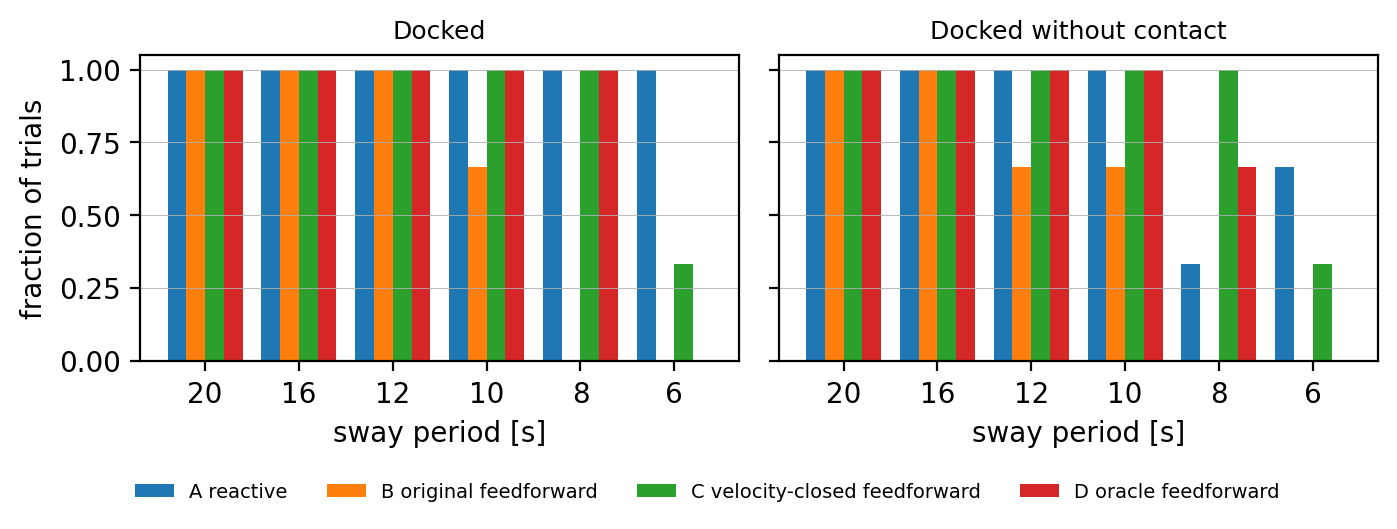
\includegraphics[width=0.88\columnwidth]{figures/success_vs_period.png}}
  \caption{Docking success versus sway period on one host, three trials per cell (six for arm B and four for arm C at 8~s). Left: latched. Right: latched without crossing the aperture boundary.}
  \label{fig:success}
\end{figure}

\begin{table}[t]
  \caption{Core sweep, 76 trials. Docked (of which without contact) out of three trials per cell unless stated; median over the cell of the lateral offset at the entry plane, over the trials that crossed it; median time to seat over the docked trials. Generated from the per-trial metrics by the same script as Figs.~\ref{fig:success} to~\ref{fig:capture}.}
  \label{tab:core}
  \centering
  \footnotesize\setlength{\tabcolsep}{2.6pt}
  \begin{tabular}{@{}lcccccc@{}}
    \toprule
    Period [s] & 20 & 16 & 12 & 10 & 8 & 6 \\
    \midrule
    A docked (clean) & 3 (3) & 3 (3) & 3 (3) & 3 (3) & 3 (1) & 3 (2) \\
    B docked (clean) & 3 (3) & 3 (3) & 3 (2) & 2 (2) & 0 of 6 & 0 \\
    C docked (clean) & 3 (3) & 3 (3) & 3 (3) & 3 (3) & 4 (4) of 4 & 1 (1) \\
    D docked (clean) & 3 (3) & 3 (3) & 3 (3) & 3 (3) & 3 (2) & 0 \\
    \midrule
    A offset [cm] & 0.5 & 0.7 & 0.2 & 0.7 & 2.1 & 3.4 \\
    B offset [cm] & 2.1 & 3.6 & 1.4 & 0.3 & 4.3 & 2.4 \\
    C offset [cm] & 0.3 & 0.6 & 0.4 & 0.5 & 1.6 & 1.7 \\
    D offset [cm] & 1.9 & 4.2 & 2.5 & 3.4 & 2.4 & 5.7 \\
    \midrule
    A seat time [s] & 18 & 20 & 20 & 22 & 80 & 76 \\
    B seat time [s] & 23 & 27 & 34 & 37 & -- & -- \\
    C seat time [s] & 39 & 45 & 42 & 42 & 47 & 156 \\
    D seat time [s] & 29 & 27 & 34 & 37 & 56 & -- \\
    \bottomrule
  \end{tabular}
\end{table}

\subsection{Over-swing against the loop model}

Fig.~\ref{fig:overswing} plots the vehicle-to-dock lateral amplitude ratio, taken over the samples with a marker measurement, against sway frequency, with the loop model of Section~\ref{sec:failure} evaluated on the identified plant ($g = 2.7$, $T = 0.4$~s) and the fine-phase position gains. The original feedforward and the oracle lie on the same curve, 1.0 at 20~s rising to 1.6 at 8~s and 1.8 to 1.9 at 6~s, within the phase-to-phase spread of each other at every period. The model at unit feedforward gain reproduces the slope and the short-period values (1.47 predicted against 1.5 to 1.7 measured at 8~s; 1.67 against 1.7 to 1.9 at 6~s) and over-predicts by about 0.1 at the long periods, where the coarse-phase ramp holds the feedforward below unit gain for part of each window. Since the oracle feeds the true velocity, the coincidence of the two curves places the over-swing in the open-loop law and the plant, not in the estimate. The reactive baseline and the velocity-closed feedforward sit at 0.9 to 1.1 at every period; the velocity loop tracks the dock at ratio 1.0 to 1.2 with the phase lag its bandwidth implies (14$^\circ$ at 8~s and 21$^\circ$ at 6~s measured, against 19 and 24$^\circ$ designed).

\begin{figure}[t]
  \centerline{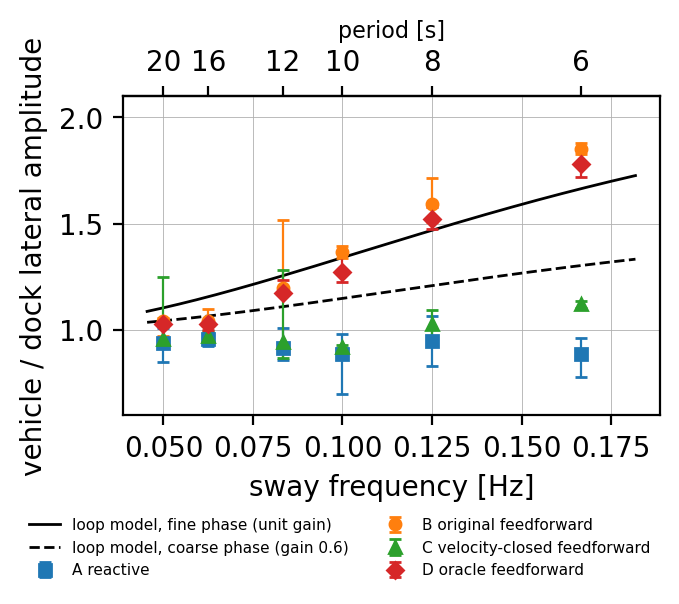
\includegraphics[width=0.82\columnwidth]{figures/overswing_vs_frequency.png}}
  \caption{Vehicle-to-dock lateral amplitude ratio, the ratio of lateral standard deviations over the samples with a marker measurement (median and range over phases), against the loop model of Section~\ref{sec:failure} on the identified plant, at unit feedforward gain (fine phase) and 0.6 (coarse phase).}
  \label{fig:overswing}
\end{figure}

\subsection{Capture quality and time to seat}

The offset at the entry plane and the time to seat (Fig.~\ref{fig:capture}, Table~\ref{tab:core}) separate the arms that dock. The velocity-closed feedforward has the smallest offsets from 12~s down, 0.4 to 1.7~cm median against the baseline's 0.8 to 4.4~cm, and holds the seat tolerance at every period. The oracle, with the true velocity but the open-loop law, seats with 2 to 6~cm offsets from 16~s, larger than the baseline's at every period but 8~s: an accurate feedforward through a mis-scaled law is worse at the entry plane than none. The baseline is the fastest to seat, 17 to 25~s from 20 to 10~s, because it closes directly on the dock and rides the swing; the velocity-closed arm takes 40 to 60~s, following the dock at the standoff until the handoff gate latches, and 156~s at 6~s.

\begin{figure}[t]
  \centerline{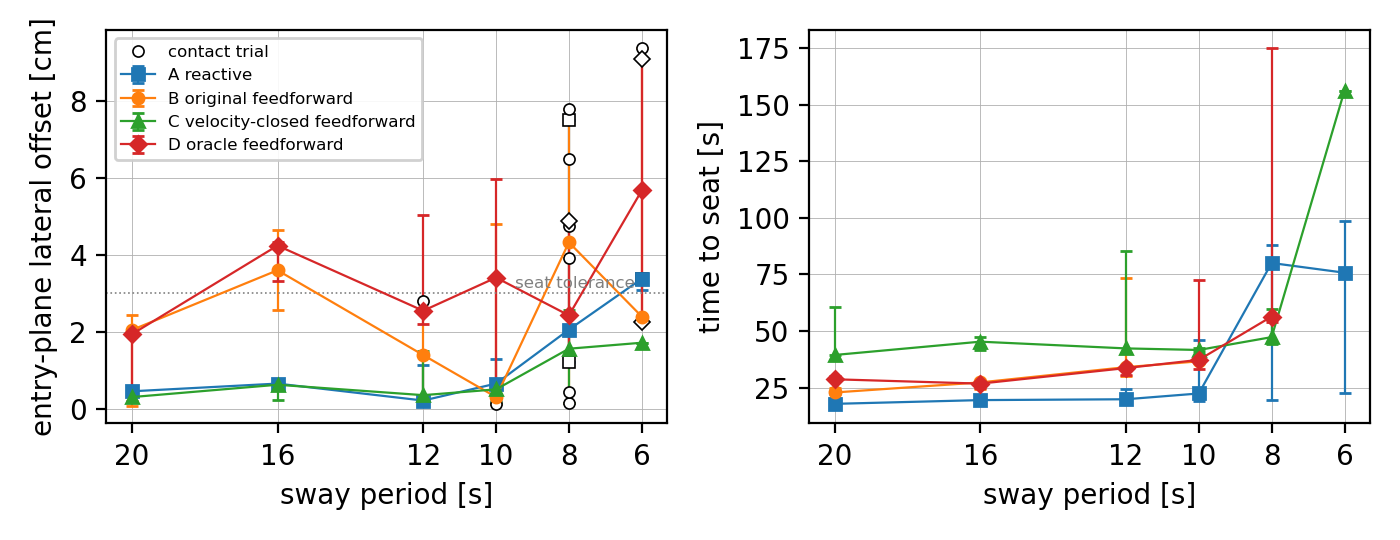
\includegraphics[width=0.92\columnwidth]{figures/capture_and_time.png}}
  \caption{Median and range over the cell of the lateral offset at the entry plane (left; hollow markers are the individual trials scored as contacts) and of the time to seat (right, docked trials only; a line is broken where no trial docked).}
  \label{fig:capture}
\end{figure}

The 6~s limit of the velocity-closed arm is the coarse handoff, not tracking. In the two trials that timed out the vehicle held the standoff for the whole run with the relative error at 2.8 to 3.2~cm RMS, the estimate on the dock to 0.4~cm and the velocity state at ratio 0.96 to 1.06; the vehicle followed the dock at ratio 1.16 with 21$^\circ$ of lag, and the residual relative velocity kept the handoff's velocity-match test from latching for ten consecutive cycles. The phase that docked did so after 156~s at the standoff. The limit moves with the loop bandwidth or the gate design, not with the estimator.

\subsection{Estimators and controllers under navigation error}

Replaying both estimators offline on the recorded measurement streams of four arm-B trials (20, 12, 10 and 8~s) with the navigation corrupted at the three levels, three seeds each, the slow part of the dock-velocity error equals the injected bias for both (0.011 to 0.070~m/s against a bias of 0.008 to 0.077~m/s, correlation 0.6 to 0.9): a camera measuring relative position cannot separate a slow vehicle-velocity error from dock velocity in either frame. The relative frame removes only the fast part, 1.3 to 1.6~cm/s against 4.0 to 4.3~cm/s for the world-frame filter, which differentiates the white position error of the navigation into its velocity state; the relative position error the controllers act on is 3.5 to 3.7~cm RMS for both.

The live sweep feeds the corrupted navigation to the controllers as well as the estimators: arms A, B and C at 10 and 8~s, three bias levels and three phases, 54 trials (Fig.~\ref{fig:nav}). The three arms separate on the bias. The reactive arm docks in 3 of 18 trials, two of them at the low level: its constant-position filter cannot follow a navigation frame that drifts even at 1~cm/s, so the relative geometry it regulates is wrong by tens of centimetres and the standoff is never satisfied. The original feedforward docks in 4 of 18, all at the low level; at the medium level its constant-velocity filter absorbs the drift as dock velocity, the open-loop law drives the vehicle at the dock velocity plus the bias, and four of six trials left the dock altogether, climbing toward the surface until the run was abandoned. The velocity-closed feedforward docks in 17 of 18, including five of six at the high level, because the bias enters the setpoint and the measured vehicle velocity alike and cancels in the loop error. Its one miss is at the high level and marks where the fix meets the estimator's own limit: with a 10~cm/s drift the world-frame filter must carry sway plus drift, above its 0.2~m/s velocity bound about 30~percent of the time, so the velocity state sits on the bound and the relative error grows to 10~cm RMS at 10~s. All three 10~s cells at that level were marginal; two seated at 106 and 112~s and the third was demoted from the fine phase at 106~s. The bound was sized for dock motion, not for a drifting frame, and is kept fixed across arms here.

\begin{figure}[t]
  \centerline{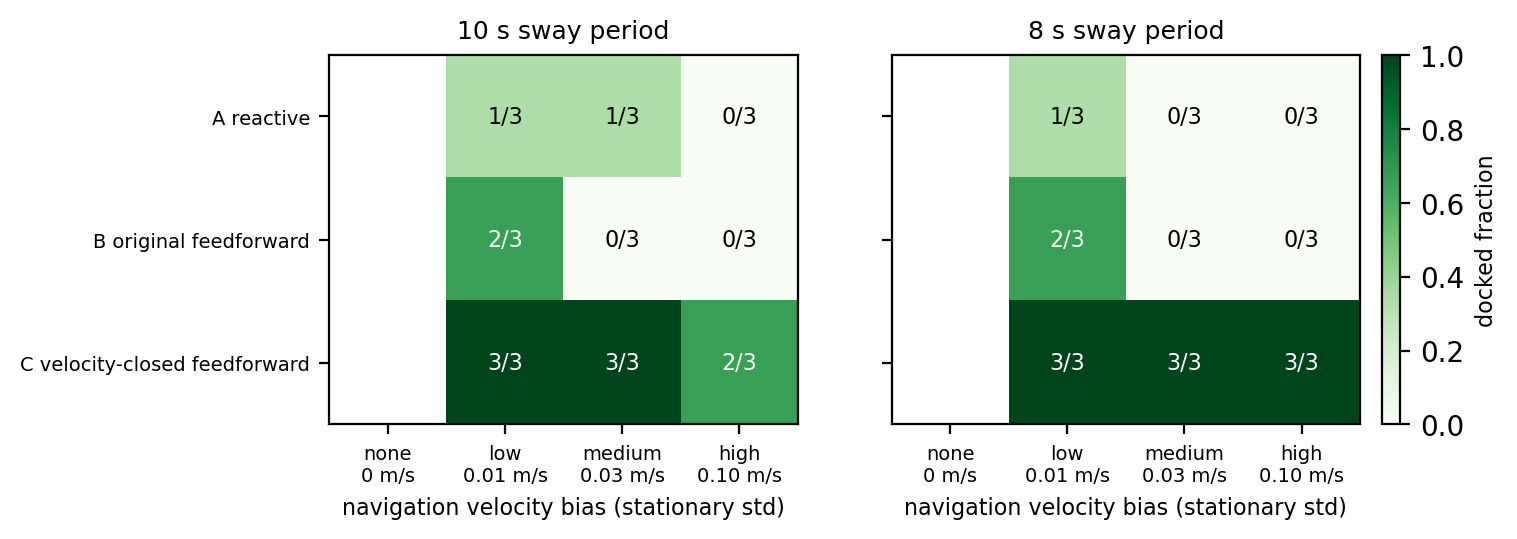
\includegraphics[width=0.92\columnwidth]{figures/nav_heatmap.png}}
  \caption{Docked fraction under first-order Gauss-Markov navigation error ($\tau_b = 30$~s, 1~mm white position noise) by arm and bias level, three phases per cell; the level-none column is the core sweep.}
  \label{fig:nav}
\end{figure}

